% Created by tikzDevice version 0.12.6 on 2026-07-03 11:54:52
% !TEX encoding = UTF-8 Unicode
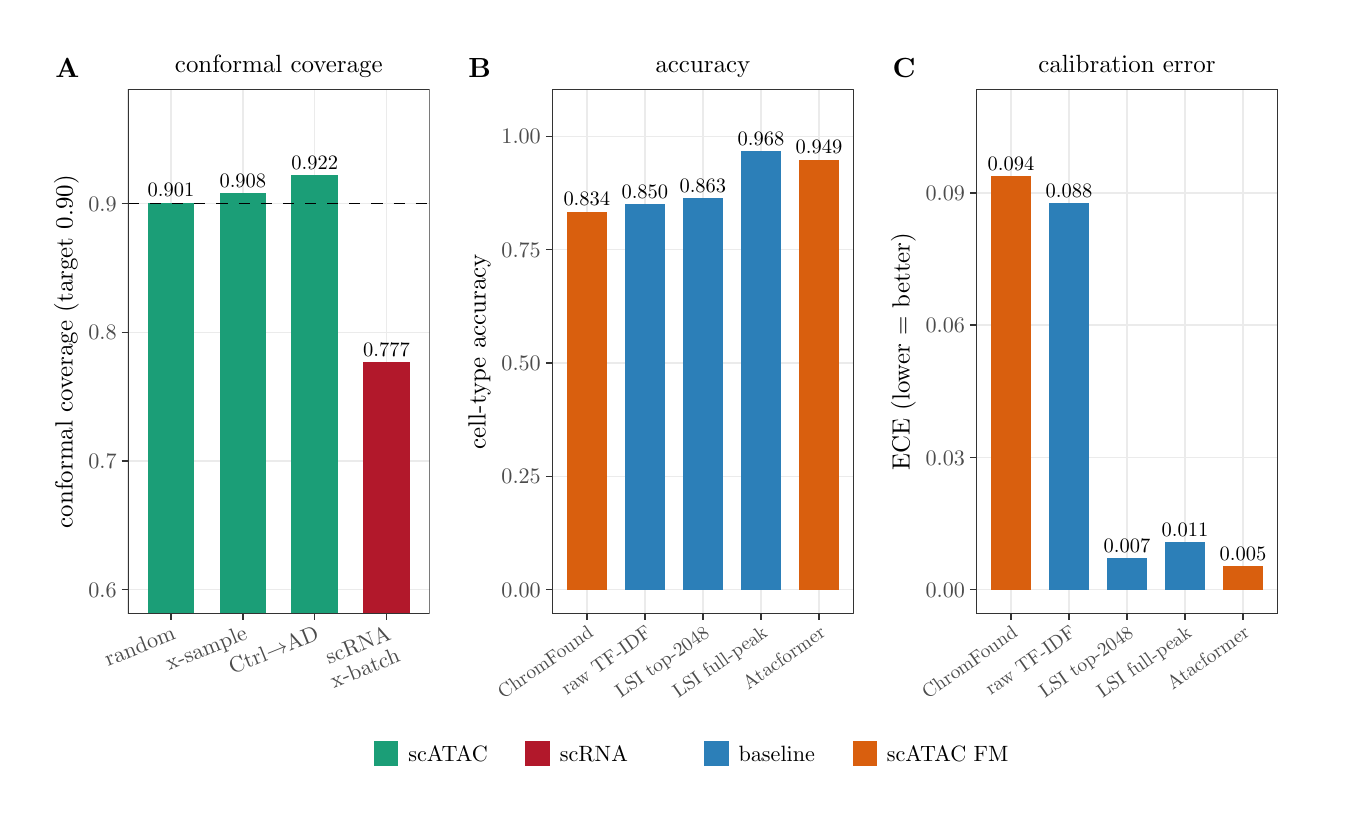
\begin{tikzpicture}[x=1pt,y=1pt]
\definecolor{fillColor}{RGB}{255,255,255}
\path[use as bounding box,fill=fillColor,fill opacity=0.00] (0,0) rectangle (469.75,281.85);
\begin{scope}
\path[clip] (  0.00,  0.00) rectangle (469.75,281.85);
\definecolor{drawColor}{RGB}{255,255,255}
\definecolor{fillColor}{RGB}{255,255,255}

\path[draw=drawColor,line width= 0.5pt,line join=round,line cap=round,fill=fillColor] (  0.00,  0.00) rectangle (469.75,281.85);
\end{scope}
\begin{scope}
\path[clip] (  5.00,  5.00) rectangle (154.25,276.85);
\definecolor{drawColor}{RGB}{255,255,255}
\definecolor{fillColor}{RGB}{255,255,255}

\path[draw=drawColor,line width= 0.5pt,line join=round,line cap=round,fill=fillColor] (  5.00,  5.00) rectangle (154.25,276.85);
\end{scope}
\begin{scope}
\path[clip] (154.25,  5.00) rectangle (307.50,276.85);
\definecolor{drawColor}{RGB}{255,255,255}
\definecolor{fillColor}{RGB}{255,255,255}

\path[draw=drawColor,line width= 0.5pt,line join=round,line cap=round,fill=fillColor] (154.25,  5.00) rectangle (307.50,276.85);
\end{scope}
\begin{scope}
\path[clip] (307.50,  5.00) rectangle (460.76,276.85);
\definecolor{drawColor}{RGB}{255,255,255}
\definecolor{fillColor}{RGB}{255,255,255}

\path[draw=drawColor,line width= 0.5pt,line join=round,line cap=round,fill=fillColor] (307.50,  5.00) rectangle (460.75,276.85);
\end{scope}
\begin{scope}
\path[clip] ( 36.22, 70.16) rectangle (145.25,259.40);
\definecolor{fillColor}{RGB}{255,255,255}

\path[fill=fillColor] ( 36.22, 70.16) rectangle (145.25,259.40);
\definecolor{drawColor}{gray}{0.92}

\path[draw=drawColor,line width= 0.5pt,line join=round] ( 36.22, 78.76) --
	(145.25, 78.76);

\path[draw=drawColor,line width= 0.5pt,line join=round] ( 36.22,125.26) --
	(145.25,125.26);

\path[draw=drawColor,line width= 0.5pt,line join=round] ( 36.22,171.75) --
	(145.25,171.75);

\path[draw=drawColor,line width= 0.5pt,line join=round] ( 36.22,218.25) --
	(145.25,218.25);

\path[draw=drawColor,line width= 0.5pt,line join=round] ( 51.80, 70.16) --
	( 51.80,259.40);

\path[draw=drawColor,line width= 0.5pt,line join=round] ( 77.76, 70.16) --
	( 77.76,259.40);

\path[draw=drawColor,line width= 0.5pt,line join=round] (103.72, 70.16) --
	(103.72,259.40);

\path[draw=drawColor,line width= 0.5pt,line join=round] (129.68, 70.16) --
	(129.68,259.40);
\definecolor{fillColor}{RGB}{27,158,119}

\path[fill=fillColor] ( 43.36,-200.23) rectangle ( 60.23,218.67);

\path[fill=fillColor] ( 69.32,-200.23) rectangle ( 86.19,222.02);

\path[fill=fillColor] ( 95.28,-200.23) rectangle (112.15,228.53);
\definecolor{fillColor}{RGB}{178,24,43}

\path[fill=fillColor] (121.24,-200.23) rectangle (138.11,161.06);
\definecolor{drawColor}{RGB}{0,0,0}

\path[draw=drawColor,line width= 0.5pt,dash pattern=on 4pt off 4pt ,line join=round] ( 36.22,218.25) -- (145.25,218.25);

\node[text=drawColor,anchor=base,inner sep=0pt, outer sep=0pt, scale=  0.74] at ( 51.80,220.71) {0.901};

\node[text=drawColor,anchor=base,inner sep=0pt, outer sep=0pt, scale=  0.74] at ( 77.76,224.06) {0.908};

\node[text=drawColor,anchor=base,inner sep=0pt, outer sep=0pt, scale=  0.74] at (103.72,230.57) {0.922};

\node[text=drawColor,anchor=base,inner sep=0pt, outer sep=0pt, scale=  0.74] at (129.68,163.10) {0.777};
\definecolor{drawColor}{gray}{0.20}

\path[draw=drawColor,line width= 0.5pt,line join=round,line cap=round] ( 36.22, 70.16) rectangle (145.25,259.40);
\end{scope}
\begin{scope}
\path[clip] (  0.00,  0.00) rectangle (469.75,281.85);
\definecolor{drawColor}{gray}{0.30}

\node[text=drawColor,anchor=base east,inner sep=0pt, outer sep=0pt, scale=  0.80] at ( 32.17, 76.00) {0.6};

\node[text=drawColor,anchor=base east,inner sep=0pt, outer sep=0pt, scale=  0.80] at ( 32.17,122.50) {0.7};

\node[text=drawColor,anchor=base east,inner sep=0pt, outer sep=0pt, scale=  0.80] at ( 32.17,169.00) {0.8};

\node[text=drawColor,anchor=base east,inner sep=0pt, outer sep=0pt, scale=  0.80] at ( 32.17,215.50) {0.9};
\end{scope}
\begin{scope}
\path[clip] (  0.00,  0.00) rectangle (469.75,281.85);
\definecolor{drawColor}{gray}{0.20}

\path[draw=drawColor,line width= 0.5pt,line join=round] ( 33.97, 78.76) --
	( 36.22, 78.76);

\path[draw=drawColor,line width= 0.5pt,line join=round] ( 33.97,125.26) --
	( 36.22,125.26);

\path[draw=drawColor,line width= 0.5pt,line join=round] ( 33.97,171.75) --
	( 36.22,171.75);

\path[draw=drawColor,line width= 0.5pt,line join=round] ( 33.97,218.25) --
	( 36.22,218.25);
\end{scope}
\begin{scope}
\path[clip] (  0.00,  0.00) rectangle (469.75,281.85);
\definecolor{drawColor}{gray}{0.20}

\path[draw=drawColor,line width= 0.5pt,line join=round] ( 51.80, 67.91) --
	( 51.80, 70.16);

\path[draw=drawColor,line width= 0.5pt,line join=round] ( 77.76, 67.91) --
	( 77.76, 70.16);

\path[draw=drawColor,line width= 0.5pt,line join=round] (103.72, 67.91) --
	(103.72, 70.16);

\path[draw=drawColor,line width= 0.5pt,line join=round] (129.68, 67.91) --
	(129.68, 70.16);
\end{scope}
\begin{scope}
\path[clip] (  0.00,  0.00) rectangle (469.75,281.85);
\definecolor{drawColor}{gray}{0.30}

\node[text=drawColor,rotate= 22.00,anchor=base east,inner sep=0pt, outer sep=0pt, scale=  0.80] at ( 53.86, 61.00) {random};

\node[text=drawColor,rotate= 22.00,anchor=base east,inner sep=0pt, outer sep=0pt, scale=  0.80] at ( 79.82, 61.00) {x-sample};

\node[text=drawColor,rotate= 22.00,anchor=base east,inner sep=0pt, outer sep=0pt, scale=  0.80] at (105.78, 61.00) {Ctrl$\to$AD};

\node[text=drawColor,rotate= 22.00,anchor=base east,inner sep=0pt, outer sep=0pt, scale=  0.80] at (131.74, 61.00) {scRNA};

\node[text=drawColor,rotate= 22.00,anchor=base east,inner sep=0pt, outer sep=0pt, scale=  0.80] at (134.98, 52.99) {x-batch};
\end{scope}
\begin{scope}
\path[clip] (  0.00,  0.00) rectangle (469.75,281.85);
\definecolor{drawColor}{RGB}{0,0,0}

\node[text=drawColor,rotate= 90.00,anchor=base,inner sep=0pt, outer sep=0pt, scale=  0.90] at ( 16.20,164.78) {conformal coverage (target 0.90)};
\end{scope}
\begin{scope}
\path[clip] (  0.00,  0.00) rectangle (469.75,281.85);
\definecolor{drawColor}{RGB}{0,0,0}

\node[text=drawColor,anchor=base,inner sep=0pt, outer sep=0pt, scale=  0.90] at ( 90.74,265.65) {conformal coverage};
\end{scope}
\begin{scope}
\path[clip] (  0.00,  0.00) rectangle (469.75,281.85);
\definecolor{drawColor}{RGB}{0,0,0}

\node[text=drawColor,anchor=base,inner sep=0pt, outer sep=0pt, scale=  1.00] at ( 14.35,263.89) {\bfseries A};
\end{scope}
\begin{scope}
\path[clip] (189.47, 70.16) rectangle (298.50,259.40);
\definecolor{fillColor}{RGB}{255,255,255}

\path[fill=fillColor] (189.47, 70.16) rectangle (298.50,259.40);
\definecolor{drawColor}{gray}{0.92}

\path[draw=drawColor,line width= 0.5pt,line join=round] (189.47, 78.76) --
	(298.50, 78.76);

\path[draw=drawColor,line width= 0.5pt,line join=round] (189.47,119.72) --
	(298.50,119.72);

\path[draw=drawColor,line width= 0.5pt,line join=round] (189.47,160.68) --
	(298.50,160.68);

\path[draw=drawColor,line width= 0.5pt,line join=round] (189.47,201.65) --
	(298.50,201.65);

\path[draw=drawColor,line width= 0.5pt,line join=round] (189.47,242.61) --
	(298.50,242.61);

\path[draw=drawColor,line width= 0.5pt,line join=round] (202.05, 70.16) --
	(202.05,259.40);

\path[draw=drawColor,line width= 0.5pt,line join=round] (223.02, 70.16) --
	(223.02,259.40);

\path[draw=drawColor,line width= 0.5pt,line join=round] (243.99, 70.16) --
	(243.99,259.40);

\path[draw=drawColor,line width= 0.5pt,line join=round] (264.96, 70.16) --
	(264.96,259.40);

\path[draw=drawColor,line width= 0.5pt,line join=round] (285.92, 70.16) --
	(285.92,259.40);
\definecolor{fillColor}{RGB}{217,95,14}

\path[fill=fillColor] (194.72, 78.76) rectangle (209.39,215.39);
\definecolor{fillColor}{RGB}{44,127,184}

\path[fill=fillColor] (215.68, 78.76) rectangle (230.36,218.08);

\path[fill=fillColor] (236.65, 78.76) rectangle (251.33,220.14);

\path[fill=fillColor] (257.62, 78.76) rectangle (272.29,237.38);
\definecolor{fillColor}{RGB}{217,95,14}

\path[fill=fillColor] (278.58, 78.76) rectangle (293.26,234.19);
\definecolor{drawColor}{RGB}{0,0,0}

\node[text=drawColor,anchor=base,inner sep=0pt, outer sep=0pt, scale=  0.74] at (202.05,217.43) {0.834};

\node[text=drawColor,anchor=base,inner sep=0pt, outer sep=0pt, scale=  0.74] at (223.02,220.12) {0.850};

\node[text=drawColor,anchor=base,inner sep=0pt, outer sep=0pt, scale=  0.74] at (243.99,222.18) {0.863};

\node[text=drawColor,anchor=base,inner sep=0pt, outer sep=0pt, scale=  0.74] at (264.96,239.42) {0.968};

\node[text=drawColor,anchor=base,inner sep=0pt, outer sep=0pt, scale=  0.74] at (285.92,236.23) {0.949};
\definecolor{drawColor}{gray}{0.20}

\path[draw=drawColor,line width= 0.5pt,line join=round,line cap=round] (189.47, 70.16) rectangle (298.50,259.40);
\end{scope}
\begin{scope}
\path[clip] (  0.00,  0.00) rectangle (469.75,281.85);
\definecolor{drawColor}{gray}{0.30}

\node[text=drawColor,anchor=base east,inner sep=0pt, outer sep=0pt, scale=  0.80] at (185.42, 76.00) {0.00};

\node[text=drawColor,anchor=base east,inner sep=0pt, outer sep=0pt, scale=  0.80] at (185.42,116.97) {0.25};

\node[text=drawColor,anchor=base east,inner sep=0pt, outer sep=0pt, scale=  0.80] at (185.42,157.93) {0.50};

\node[text=drawColor,anchor=base east,inner sep=0pt, outer sep=0pt, scale=  0.80] at (185.42,198.89) {0.75};

\node[text=drawColor,anchor=base east,inner sep=0pt, outer sep=0pt, scale=  0.80] at (185.42,239.85) {1.00};
\end{scope}
\begin{scope}
\path[clip] (  0.00,  0.00) rectangle (469.75,281.85);
\definecolor{drawColor}{gray}{0.20}

\path[draw=drawColor,line width= 0.5pt,line join=round] (187.22, 78.76) --
	(189.47, 78.76);

\path[draw=drawColor,line width= 0.5pt,line join=round] (187.22,119.72) --
	(189.47,119.72);

\path[draw=drawColor,line width= 0.5pt,line join=round] (187.22,160.68) --
	(189.47,160.68);

\path[draw=drawColor,line width= 0.5pt,line join=round] (187.22,201.65) --
	(189.47,201.65);

\path[draw=drawColor,line width= 0.5pt,line join=round] (187.22,242.61) --
	(189.47,242.61);
\end{scope}
\begin{scope}
\path[clip] (  0.00,  0.00) rectangle (469.75,281.85);
\definecolor{drawColor}{gray}{0.20}

\path[draw=drawColor,line width= 0.5pt,line join=round] (202.05, 67.91) --
	(202.05, 70.16);

\path[draw=drawColor,line width= 0.5pt,line join=round] (223.02, 67.91) --
	(223.02, 70.16);

\path[draw=drawColor,line width= 0.5pt,line join=round] (243.99, 67.91) --
	(243.99, 70.16);

\path[draw=drawColor,line width= 0.5pt,line join=round] (264.96, 67.91) --
	(264.96, 70.16);

\path[draw=drawColor,line width= 0.5pt,line join=round] (285.92, 67.91) --
	(285.92, 70.16);
\end{scope}
\begin{scope}
\path[clip] (  0.00,  0.00) rectangle (469.75,281.85);
\definecolor{drawColor}{gray}{0.30}

\node[text=drawColor,rotate= 35.00,anchor=base east,inner sep=0pt, outer sep=0pt, scale=  0.70] at (204.82, 62.16) {ChromFound};

\node[text=drawColor,rotate= 35.00,anchor=base east,inner sep=0pt, outer sep=0pt, scale=  0.70] at (225.79, 62.16) {raw TF-IDF};

\node[text=drawColor,rotate= 35.00,anchor=base east,inner sep=0pt, outer sep=0pt, scale=  0.70] at (246.75, 62.16) {LSI top-2048};

\node[text=drawColor,rotate= 35.00,anchor=base east,inner sep=0pt, outer sep=0pt, scale=  0.70] at (267.72, 62.16) {LSI full-peak};

\node[text=drawColor,rotate= 35.00,anchor=base east,inner sep=0pt, outer sep=0pt, scale=  0.70] at (288.69, 62.16) {Atacformer};
\end{scope}
\begin{scope}
\path[clip] (  0.00,  0.00) rectangle (469.75,281.85);
\definecolor{drawColor}{RGB}{0,0,0}

\node[text=drawColor,rotate= 90.00,anchor=base,inner sep=0pt, outer sep=0pt, scale=  0.90] at (165.45,164.78) {cell-type accuracy};
\end{scope}
\begin{scope}
\path[clip] (  0.00,  0.00) rectangle (469.75,281.85);
\definecolor{drawColor}{RGB}{0,0,0}

\node[text=drawColor,anchor=base,inner sep=0pt, outer sep=0pt, scale=  0.90] at (243.99,265.65) {accuracy};
\end{scope}
\begin{scope}
\path[clip] (  0.00,  0.00) rectangle (469.75,281.85);
\definecolor{drawColor}{RGB}{0,0,0}

\node[text=drawColor,anchor=base,inner sep=0pt, outer sep=0pt, scale=  1.00] at (163.34,263.89) {\bfseries B};
\end{scope}
\begin{scope}
\path[clip] (342.73, 70.16) rectangle (451.76,259.40);
\definecolor{fillColor}{RGB}{255,255,255}

\path[fill=fillColor] (342.73, 70.16) rectangle (451.76,259.40);
\definecolor{drawColor}{gray}{0.92}

\path[draw=drawColor,line width= 0.5pt,line join=round] (342.73, 78.76) --
	(451.76, 78.76);

\path[draw=drawColor,line width= 0.5pt,line join=round] (342.73,126.55) --
	(451.76,126.55);

\path[draw=drawColor,line width= 0.5pt,line join=round] (342.73,174.34) --
	(451.76,174.34);

\path[draw=drawColor,line width= 0.5pt,line join=round] (342.73,222.13) --
	(451.76,222.13);

\path[draw=drawColor,line width= 0.5pt,line join=round] (355.31, 70.16) --
	(355.31,259.40);

\path[draw=drawColor,line width= 0.5pt,line join=round] (376.27, 70.16) --
	(376.27,259.40);

\path[draw=drawColor,line width= 0.5pt,line join=round] (397.24, 70.16) --
	(397.24,259.40);

\path[draw=drawColor,line width= 0.5pt,line join=round] (418.21, 70.16) --
	(418.21,259.40);

\path[draw=drawColor,line width= 0.5pt,line join=round] (439.17, 70.16) --
	(439.17,259.40);
\definecolor{fillColor}{RGB}{217,95,14}

\path[fill=fillColor] (347.97, 78.76) rectangle (362.64,228.34);
\definecolor{fillColor}{RGB}{44,127,184}

\path[fill=fillColor] (368.93, 78.76) rectangle (383.61,218.62);

\path[fill=fillColor] (389.90, 78.76) rectangle (404.58, 90.07);

\path[fill=fillColor] (410.87, 78.76) rectangle (425.55, 95.96);
\definecolor{fillColor}{RGB}{217,95,14}

\path[fill=fillColor] (431.84, 78.76) rectangle (446.51, 87.20);
\definecolor{drawColor}{RGB}{0,0,0}

\node[text=drawColor,anchor=base,inner sep=0pt, outer sep=0pt, scale=  0.74] at (355.31,230.38) {0.094};

\node[text=drawColor,anchor=base,inner sep=0pt, outer sep=0pt, scale=  0.74] at (376.27,220.66) {0.088};

\node[text=drawColor,anchor=base,inner sep=0pt, outer sep=0pt, scale=  0.74] at (397.24, 92.11) {0.007};

\node[text=drawColor,anchor=base,inner sep=0pt, outer sep=0pt, scale=  0.74] at (418.21, 98.00) {0.011};

\node[text=drawColor,anchor=base,inner sep=0pt, outer sep=0pt, scale=  0.74] at (439.17, 89.24) {0.005};
\definecolor{drawColor}{gray}{0.20}

\path[draw=drawColor,line width= 0.5pt,line join=round,line cap=round] (342.73, 70.16) rectangle (451.76,259.40);
\end{scope}
\begin{scope}
\path[clip] (  0.00,  0.00) rectangle (469.75,281.85);
\definecolor{drawColor}{gray}{0.30}

\node[text=drawColor,anchor=base east,inner sep=0pt, outer sep=0pt, scale=  0.80] at (338.68, 76.00) {0.00};

\node[text=drawColor,anchor=base east,inner sep=0pt, outer sep=0pt, scale=  0.80] at (338.68,123.79) {0.03};

\node[text=drawColor,anchor=base east,inner sep=0pt, outer sep=0pt, scale=  0.80] at (338.68,171.58) {0.06};

\node[text=drawColor,anchor=base east,inner sep=0pt, outer sep=0pt, scale=  0.80] at (338.68,219.37) {0.09};
\end{scope}
\begin{scope}
\path[clip] (  0.00,  0.00) rectangle (469.75,281.85);
\definecolor{drawColor}{gray}{0.20}

\path[draw=drawColor,line width= 0.5pt,line join=round] (340.48, 78.76) --
	(342.73, 78.76);

\path[draw=drawColor,line width= 0.5pt,line join=round] (340.48,126.55) --
	(342.73,126.55);

\path[draw=drawColor,line width= 0.5pt,line join=round] (340.48,174.34) --
	(342.73,174.34);

\path[draw=drawColor,line width= 0.5pt,line join=round] (340.48,222.13) --
	(342.73,222.13);
\end{scope}
\begin{scope}
\path[clip] (  0.00,  0.00) rectangle (469.75,281.85);
\definecolor{drawColor}{gray}{0.20}

\path[draw=drawColor,line width= 0.5pt,line join=round] (355.31, 67.91) --
	(355.31, 70.16);

\path[draw=drawColor,line width= 0.5pt,line join=round] (376.27, 67.91) --
	(376.27, 70.16);

\path[draw=drawColor,line width= 0.5pt,line join=round] (397.24, 67.91) --
	(397.24, 70.16);

\path[draw=drawColor,line width= 0.5pt,line join=round] (418.21, 67.91) --
	(418.21, 70.16);

\path[draw=drawColor,line width= 0.5pt,line join=round] (439.17, 67.91) --
	(439.17, 70.16);
\end{scope}
\begin{scope}
\path[clip] (  0.00,  0.00) rectangle (469.75,281.85);
\definecolor{drawColor}{gray}{0.30}

\node[text=drawColor,rotate= 35.00,anchor=base east,inner sep=0pt, outer sep=0pt, scale=  0.70] at (358.07, 62.16) {ChromFound};

\node[text=drawColor,rotate= 35.00,anchor=base east,inner sep=0pt, outer sep=0pt, scale=  0.70] at (379.04, 62.16) {raw TF-IDF};

\node[text=drawColor,rotate= 35.00,anchor=base east,inner sep=0pt, outer sep=0pt, scale=  0.70] at (400.01, 62.16) {LSI top-2048};

\node[text=drawColor,rotate= 35.00,anchor=base east,inner sep=0pt, outer sep=0pt, scale=  0.70] at (420.97, 62.16) {LSI full-peak};

\node[text=drawColor,rotate= 35.00,anchor=base east,inner sep=0pt, outer sep=0pt, scale=  0.70] at (441.94, 62.16) {Atacformer};
\end{scope}
\begin{scope}
\path[clip] (  0.00,  0.00) rectangle (469.75,281.85);
\definecolor{drawColor}{RGB}{0,0,0}

\node[text=drawColor,rotate= 90.00,anchor=base,inner sep=0pt, outer sep=0pt, scale=  0.90] at (318.70,164.78) {ECE (lower = better)};
\end{scope}
\begin{scope}
\path[clip] (  0.00,  0.00) rectangle (469.75,281.85);
\definecolor{drawColor}{RGB}{0,0,0}

\node[text=drawColor,anchor=base,inner sep=0pt, outer sep=0pt, scale=  0.90] at (397.24,265.65) {calibration error};
\end{scope}
\begin{scope}
\path[clip] (  0.00,  0.00) rectangle (469.75,281.85);
\definecolor{drawColor}{RGB}{0,0,0}

\node[text=drawColor,anchor=base,inner sep=0pt, outer sep=0pt, scale=  1.00] at (316.66,263.89) {\bfseries C};
\end{scope}
\begin{scope}
\path[clip] (  0.00,  0.00) rectangle (469.75,281.85);
\definecolor{fillColor}{RGB}{255,255,255}

\path[fill=fillColor] (120.07, 10.00) rectangle (230.38, 29.00);
\end{scope}
\begin{scope}
\path[clip] (  0.00,  0.00) rectangle (469.75,281.85);
\definecolor{fillColor}{RGB}{255,255,255}

\path[fill=fillColor] (124.57, 14.50) rectangle (134.57, 24.50);
\definecolor{fillColor}{RGB}{27,158,119}

\path[fill=fillColor] (125.15, 15.08) rectangle (133.98, 23.92);
\end{scope}
\begin{scope}
\path[clip] (  0.00,  0.00) rectangle (469.75,281.85);
\definecolor{fillColor}{RGB}{255,255,255}

\path[fill=fillColor] (179.28, 14.50) rectangle (189.28, 24.50);
\definecolor{fillColor}{RGB}{178,24,43}

\path[fill=fillColor] (179.86, 15.08) rectangle (188.70, 23.92);
\end{scope}
\begin{scope}
\path[clip] (  0.00,  0.00) rectangle (469.75,281.85);
\definecolor{drawColor}{RGB}{0,0,0}

\node[text=drawColor,anchor=base west,inner sep=0pt, outer sep=0pt, scale=  0.80] at (137.57, 16.74) {scATAC};
\end{scope}
\begin{scope}
\path[clip] (  0.00,  0.00) rectangle (469.75,281.85);
\definecolor{drawColor}{RGB}{0,0,0}

\node[text=drawColor,anchor=base west,inner sep=0pt, outer sep=0pt, scale=  0.80] at (192.28, 16.74) {scRNA};
\end{scope}
\begin{scope}
\path[clip] (  0.00,  0.00) rectangle (469.75,281.85);
\definecolor{fillColor}{RGB}{255,255,255}

\path[fill=fillColor] (239.38, 10.00) rectangle (367.91, 29.00);
\end{scope}
\begin{scope}
\path[clip] (  0.00,  0.00) rectangle (469.75,281.85);
\definecolor{fillColor}{RGB}{255,255,255}

\path[fill=fillColor] (243.88, 14.50) rectangle (253.88, 24.50);
\definecolor{fillColor}{RGB}{44,127,184}

\path[fill=fillColor] (244.46, 15.08) rectangle (253.30, 23.92);
\end{scope}
\begin{scope}
\path[clip] (  0.00,  0.00) rectangle (469.75,281.85);
\definecolor{fillColor}{RGB}{255,255,255}

\path[fill=fillColor] (297.48, 14.50) rectangle (307.48, 24.50);
\definecolor{fillColor}{RGB}{217,95,14}

\path[fill=fillColor] (298.06, 15.08) rectangle (306.90, 23.92);
\end{scope}
\begin{scope}
\path[clip] (  0.00,  0.00) rectangle (469.75,281.85);
\definecolor{drawColor}{RGB}{0,0,0}

\node[text=drawColor,anchor=base west,inner sep=0pt, outer sep=0pt, scale=  0.80] at (256.88, 16.74) {baseline};
\end{scope}
\begin{scope}
\path[clip] (  0.00,  0.00) rectangle (469.75,281.85);
\definecolor{drawColor}{RGB}{0,0,0}

\node[text=drawColor,anchor=base west,inner sep=0pt, outer sep=0pt, scale=  0.80] at (310.48, 16.74) {scATAC FM};
\end{scope}
\end{tikzpicture}
